% Semantic Assistants - http://www.semanticsoftware.info/semantic-assistants
%
% This file is part of the Semantic Assistants architecture.
%
% Copyright (C) 2012, 2013 Semantic Software Lab, http://www.semanticsoftware.info
% The Semantic Assistants architecture is free software: you can
% redistribute and/or modify it under the terms of the GNU Affero General
% Public License as published by the Free Software Foundation, either
% version 3 of the License, or (at your option) any later version.
%   
% This program is distributed in the hope that it will be useful,
% but WITHOUT ANY WARRANTY; without even the implied warranty of
% MERCHANTABILITY or FITNESS FOR A PARTICULAR PURPOSE.  See the
% GNU Affero General Public License for more details.
% 
% You should have received a copy of the GNU Affero General Public License
% along with this program.  If not, see <http://www.gnu.org/licenses/>.

\chapter{Wiki Integration}
Wikis are web-based software applications that allow users to collaboratively create and edit web page content through a Web browser using a simplified syntax. The ease-of-use and ``open'' philosophy of wikis have brought them to the attention of organizations and online communities, leading to a wide-spread adoption as a simple and ``quick'' way of collaborative knowledge management. The \sa architecture provides an extensible wiki connector component that allows a multitude of wiki engines to connect to a \sa server and employ various NLP services on their content.

The wiki connector component is designed regardless of what underlying wiki engine intends to use the NLP services within its environment. This means that the wiki component does not have any concrete wiki engine specifications hard coded in its implementation. Rather, it provides an extensible interface so that various wiki engines can be added to its architecture with little effort.

As a concrete application, we have developed the integration of \sa with MediaWiki\footnote{MediaWiki, \url{http://www.mediawiki.org}} -- a popular wiki engine best known from the Wikipedia project. In the following sections, we will describe the SA-MediaWiki integration in details, as well as the core, reusable features of the wiki component.

\section{Features}
The ultimate goal of the Wiki-SA integration is to provide a seamless integration of NLP capabilities within a wiki environment, with the least possible modifications on its engine. Towards this end, the Wiki-SA integration adopts a collaborative approach, where a number of different components communicate with each other over standard protocols.

\subsection{Storing User Preferences} The Wiki-NLP integration communicates with a \sa server based on the values of special cookies available inside the user's browser. To store such values, the first time a user asks for the Wiki-NLP interface in the wiki, he is temporarily redirected to a different page shown in Figure~\ref{fig:wiki_config}, where the following items can be configured:

\begin{itemize}\itemsep1mm
\item The wiki engine and version
\item The base URL of the wiki\footnote{The Wiki-NLP integration tries to guess the base URL of the wiki API, based on the wiki location. You should, however, check whether the suggested address is indeed correct and uses the right capitalization. For example, ``\emph{http://localhost/mywiki}'' and ``\emph{http://localhost/MyWiki}'' are not considered the same.} (i.e., from which the wiki API can be accessed)
\item A user name and password that can be used by the Wiki-NLP integration to communicate with the wiki engine
\item The \sa server to connect to
\end{itemize}

\begin{figure}[ht]
\centering
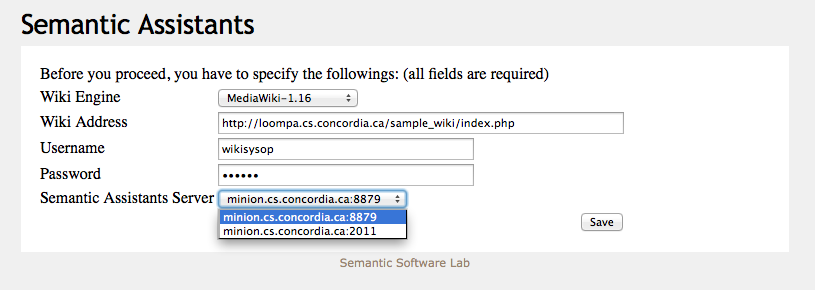
\includegraphics[width=0.9\textwidth]{pictures/wiki_config.png}
\caption{Configuring the Wiki-NLP integration}
\label{fig:wiki_config}
\end{figure}

Once the user saves the configuration, the provided information is stored in the user's browser and will remain there for the subsequent Wiki-SA interactions. Therefore, the configuration page is only shown to users once in the beginning of their session, unless the cookies are explicitly removed by the user. Clicking on the ``Save'' button will return the user to the previous page that he was viewing.

\subsection{NLP Service Invocation}
Once the configuration settings are stored in the browser, users can inquire about the available NLP services by clicking on the ``Semantic Assistants'' link inside the wiki menu bar. This action will reload the page, but this time the Wiki-NLP user interface is appended to the bottom of the current wiki page. This user interface, shown in Figure~\ref{fig:semassist_ui}, allows users to view a dynamically generated list of available assistants and add multiple wiki pages of interest to a so-called ``collection''. The list of pages in the collection is temporarily stored in the browser, hence, users can continue browsing to other pages of the wiki.

\begin{figure}
\centering
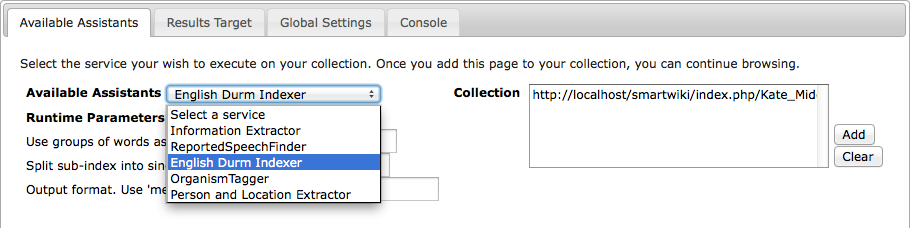
\includegraphics[width=\textwidth]{pictures/semassist_ui.png}
\caption{The Wiki-NLP interface in MediaWiki}
\label{fig:semassist_ui}
\end{figure}

\blankline
Once the collection is prepared and an assistant is selected from the list, the second tab of the Wiki-NLP interface allows users to choose where they would like the results to be stored. Illustrated in Figure~\ref{fig:semassist_target}, the current available choices in the Wiki-NLP integration are:

\begin{description}\itemsep1mm
\item [``Same Page''], i.e., the results will be written in the same page as the resource. If the user has multiple pages in the collection, each results will be written into its corresponding source page. The current options for this item are the wiki page's main ``body'', or its associated ``talk''\footnote{In some MediaWiki skins, a talk page is also known as the ``discussion'' page.} section.
\item [``Another Page''], i.e., writing the results to a different page in the wiki. If the user has multiple pages in the collection, the results of all the wiki pages will be aggregated into one output and written into the specified wiki page. In order to precisely choose a destination for this option, users have to select a namespace from a list of available namespaces in the wiki and provide a unique page name. If the specified wiki page exists in the wiki, the results will be appended to the end of the page, otherwise a new wiki page will be automatically created.
\item [``Another Wiki''], i.e., writing the results of the analysis into a different wiki than the source, provided that its engine is supported by the integration. Needless to say, users must provide the integration with (1) the address of the destination wiki, (2) its underlying wiki engine and version, (3) a valid username and password, and (4) a valid page name. Similar to the previous option, the results of the analysis will be aggregated and made persistent in the destination wiki page.
\end{description}

\begin{figure}
\centering
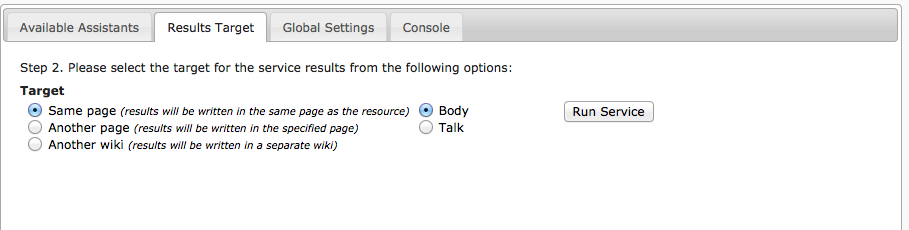
\includegraphics[width=\textwidth]{pictures/semassist_target.png}
\caption{The Wiki-NLP interface in MediaWiki}
\label{fig:semassist_target}
\end{figure}

The ``Console'' tab of the Wiki-NLP interface shows user-friendly logs of the NLP service execution and indicates where the results are written if the execution is successful.

\subsection{Global Settings}
Similar to other \sa clients, users can dynamically change which \sa server they want their wiki to connect to. The ``Global Settings'' tab in the Wiki-NLP interface, shown in Figure~\ref{fig:semassist_settings}, allows users to select a \sa server from a list of pre-defined addresses, as well as defining a custom end point. Once the user clicks the ``connect'' button, the selected server address is stored in the browser cookies and will take effect as soon as the user refreshes the browser.

\begin{figure}[h!]
\centering
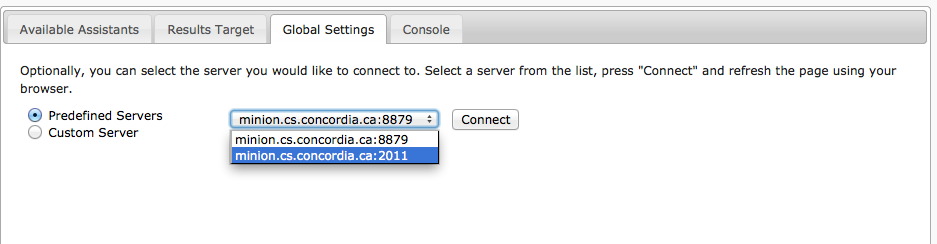
\includegraphics[width=\textwidth]{pictures/semassist_settings.png}
\caption{Global settings of the Wiki-NLP integration}
\label{fig:semassist_settings}
\end{figure}

\section{Installation}
The Wiki-SA integration is composed of two separate components: a server-side component and a wiki plug-in. While the server-side component is the same for different wiki systems, each wiki plug-in should be implemented for a specific engine. If you prefer to use the services available in our public repository, you can skip the next section and continue on to the wiki plug-in installation.

\subsection{Server-Side Component}
\label{sec:wiki_component}
In order to install the server-side component, browse to \path{Clients/Wiki} folder in the \sa folder through a terminal and type \texttt{ant pack}. This command will automatically build the server-side component as a \texttt{.WAR} file that can be deployed on any Java Servlet Container program, such as Apache Tomcat. Deploying the servlet on a container varies from one program to the other. Please consult the user guide of your container of choice for this matter.

Once the server-side is deployed and started, it is automatically published on the container's default port number. For example, if your Tomcat is configured to use port \texttt{8080} as its default port, the servlet will be accessible on \texttt{http://HOSTNAME:8080/SA-WikiConnector}.

\subsection{Wiki Plug-in}
The Wiki-SA integration needs to be introduced to the wiki through a plug-in. Here, we will provide the details of installing the \sa extension for MediaWiki, available in the \path{Clients/Wiki/MediaWiki/extension} folder. Simply copy the \texttt{\sa} folder to \path{PATH_TO_YOUR_MEDIAWIKI/extensions} folder. Next, you have to \emph{install} the extension on the wiki engine by adding the following line to the \path{LocalProperties.php} file present in the root of your MediaWiki installation folder:

\begin{figure}[h!]
\centering
\begin{lstlisting}[language=PHP,numbers=left,xleftmargin=4mm,columns=flexible]
include_once("$IP/extensions/SemanticAssistants/SemanticAssistants.php");
\end{lstlisting}
\caption{Installing the \sa extension on the MediaWiki engine}
\label{list:mediawiki_sa_extension_install}
\end{figure}

Adding this line is all that is needed to enable your wiki users to inquire and invoke NLP pipeline on the wiki content. However, the extension by default connects to the public \sa wiki component. If you have installed the server-side component described in the previous section, you have to change the default wiki component address to the servlet deployed on your container. Find the following line in \path{PATH_TO_YOUR_MEDIAWIKI/extensions/SemanticAssistants/SemanticAssistants.php} file and update it accordingly, by changing the \emph{``http://loompa.cs.concordia.ca:8080/''} entry to where your wiki component is published:

\begin{figure}[h!]
\centering
\begin{lstlisting}[language=PHP,numbers=left,xleftmargin=4mm,columns=flexible]
print("<li> <a href=\"http://loompa.cs.concordia.ca:8080/SA-WikiConnector/SemAssistServlet?action=proxy\">Semantic Assistants</a></li>");\end{lstlisting}
\caption{Configuring the \sa MediaWiki extension file}
\label{list:mediawiki_sa_extension_config}
\end{figure}

You can verify the successful installation of the \sa extension by viewing the ``\texttt{Special:Version}'' page of your wiki: The \sa extension must be listed under the ``Installed extensions'' section of the page (Figure~\ref{fig:semassist_plugin} (a)), and a ``Semantic Assistants'' link should be added to the wiki menu bar (Figure~\ref{fig:semassist_plugin} (b)).

\begin{figure}
\centering
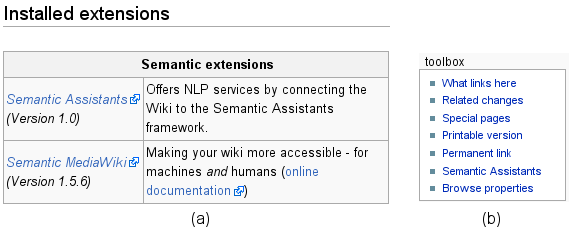
\includegraphics[scale=0.8]{pictures/semassist_plugin.png}
\caption{The \sa extension installed on MediaWiki}
\label{fig:semassist_plugin}
\end{figure}

\blankline
\noindent
\textbf{Note:} Most of the NLP services produce some sort of \emph{semantic metadata} that needs to be stored in the wiki. In our SA-MediaWiki integration, the semantic results are stored in the wiki using the Semantic MediaWiki (SMW) extension\footnote{Semantic MediaWiki Extension, \url{http://semantic-mediawiki.org}}. The SMW extension provides a special syntax to declare and query semantic metadata inside wiki pages. Therefore, installing the SMW extension is considered as a prerequisite for the SA-MediaWiki integration. The installation directions can be found on the SMW website\footnote{Semantic MediaWiki Extension Installation, \url{http://semantic-mediawiki.org/wiki/Help:Installation}}.

\subsection{Wiki Templates}
The NLP pipelines' results are made persistent in the wiki once an analysis is finished. For a more user-friendly results format, we have developed pre-defined, customizable templates in the Wiki-NLP integration that embed the generated results in a wiki table format. In order to use the templates in your MediaWiki instance, you have to import them to your wiki repository. Browse to the ``\texttt{Special Pages}'' page of your wiki and click on the ``\texttt{Import Pages}'' link under the ``\texttt{Page Tools}'' section\footnote{In the default installation of MediaWiki, permission of importing pages to the wiki is limited to users with the ``admin'' role.}. From the ``\texttt{Import XML data}'' box click on the ``\texttt{Browse}'' button and upload the \texttt{WikiNLP\_SA\_templates.xml} file located in the \path{Clients/Wiki/MediaWiki/templates} folder, as shown in Figure~\ref{fig:wiki_template_import}.

\begin{figure}
\centering
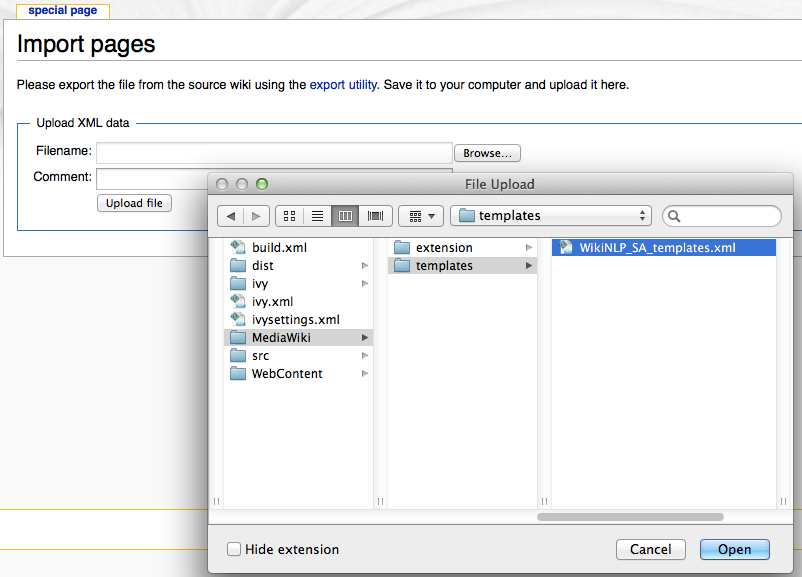
\includegraphics[width=0.9\textwidth]{pictures/wiki_template_import.png}
\caption{Importing the \sa templates ito MediaWiki}
\label{fig:wiki_template_import}
\end{figure}

Note that there are no templates for the ``File'' and ``Document'' output types (see Section~\ref{sec:response}) and the content of the generated output is written to the wiki repository as regular wiki pages.

\section{Development Notes}
In this section, we provide further details on the underlying architecture of the Wiki-NLP integration and explain how more wiki engines can be added.

\subsection{System Architecture}
As stated earlier, the Wiki-NLP architecture is a collaborative approach, combining the power of an extensible server-side component and a lightweight wiki-side plug-in. While the server-side wiki component is responsible for executing the NLP services, the wiki extension handles all the wiki-specific tasks, such as manipulating the wiki menu bar or patrolling changes in the wiki repository. In our system architecture, illustrated in Figure~\ref{fig:wikinlp_arch}, the communication between the two aforementioned components and the user's browser is carried out over the HTTP protocol using JavaScript code that is dynamically injected into the user's browser.

\begin{figure}
\centering
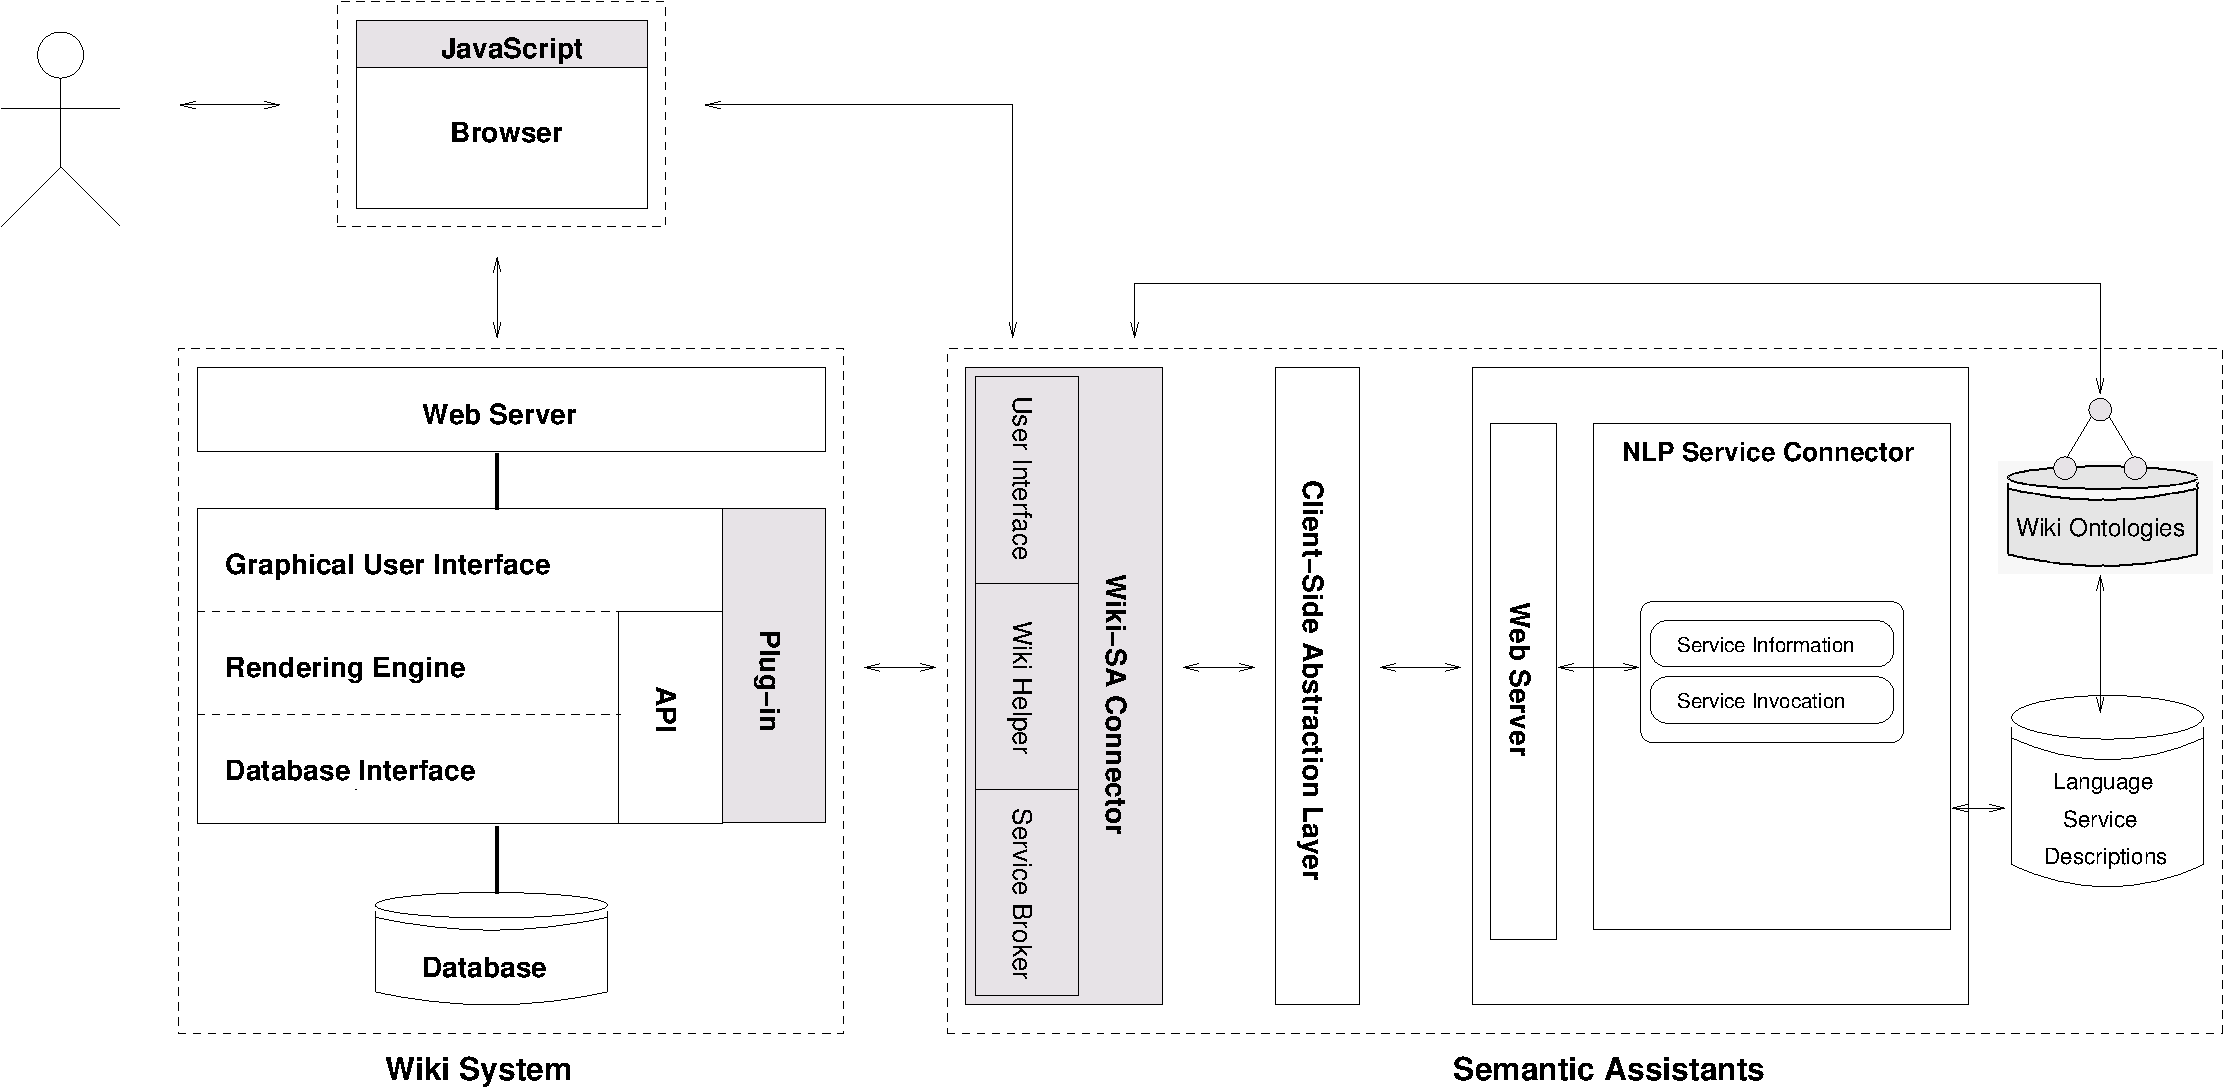
\includegraphics[width=0.9\textwidth]{pictures/wikinlp_arch}
\caption{The Wiki-NLP integration architecture}
\label{fig:wikinlp_arch}
\end{figure}

An analysis session is started when the user clicks on the \sa link in the wiki, like the one shown in Figure~\ref{fig:semassist_plugin}, or the wiki extensions makes a headless request to the wiki component. If the request parameters are not sufficient, the user is redirected to the settings page. Otherwise, the wiki component loads the requesting wiki ontology from its repository (see the next section) and generates a custom user interface based on the wiki's capabilities, e.g., its list of namespaces. The user interface is then injected into the user's browser, as shown in Figure~\ref{fig:semassist_ui}.

Once an NLP service execution request is sent to the wiki component, the service call is delegated to the designated \sa server and the results are eventually transformed and written back to the wiki repository.

\subsection{Wiki Ontologies}
In our Wiki-NLP integration, we have adopted a semantics-based approach, where different wiki engines are introduced to the integration architecture through their \emph{ontology} files. By using OWL as the ontology language to formally describe a wiki, the integration does not need to know about their concrete implementation; rather it uses automatic reasoning on their ontologies to discover each wiki's structure and capabilities.

\begin{figure}
\centering
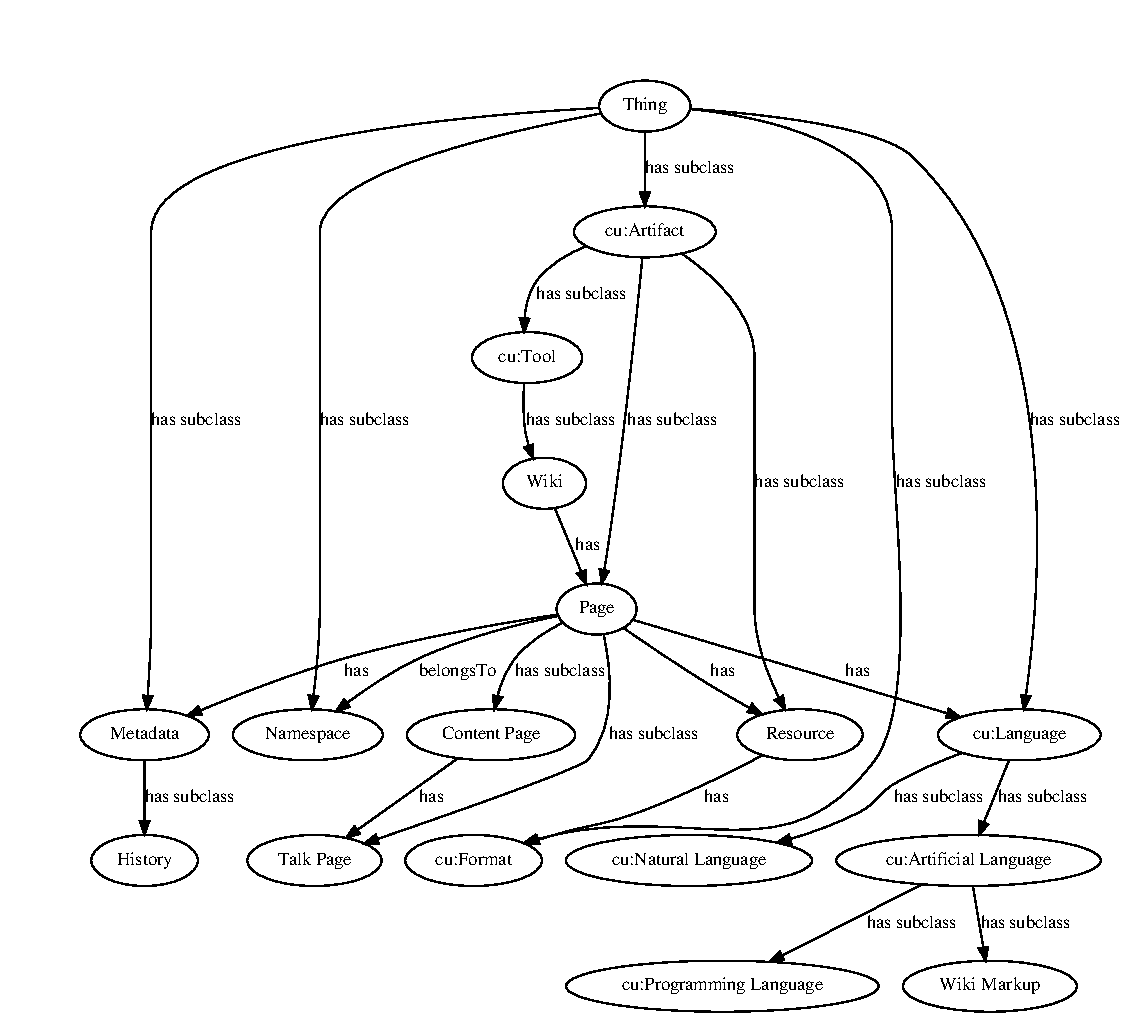
\includegraphics[scale=0.7]{pictures/wiki_onto.pdf}
\caption{Wiki Upper Ontology}
\label{fig:wiki_onto}
\end{figure}

To facilitate the process of ontology definition, we have designed a generic \emph{upper ontology} for wiki systems shown in Figure~\ref{fig:wiki_onto}, which also includes concepts defined in the \sa upper ontology (see Section~\ref{sec:sa_ontology}) -- a multi-purpose ontology that describes five core concepts to model the relationships between users, their tasks, the artifacts involved and their format and language.  

\begin{table}
\centering
\caption{Concepts in the wiki upper ontology}
\label{tab:wiki_onto_concepts}
\textsf{\small
\begin{tabular}{l l l}
  \hline 
  \textbf{Concept}&\textbf{Description} &\textbf{Example} \\
  \hline
  Wiki & \emph{wiki engine}  & MediaWiki
  \\
  Page & \emph{Wiki elements encompassing textual content} & ``Semantic Web''
  \\
  Namespace & \emph{Category names to differentiate pages at a high level}  & ``Help'', ``Project''
  \\  
  Resource & \emph{Files with arbitrary formats} & Picture.jpg
  \\
  Metadata & \emph{Metadata associated with wiki pages}  & History, Semantic Annotations
  \\
  Wiki Markup & \emph{Ontological representation of wiki syntax} & MediaWiki Markup\\
\hline
\end{tabular}}
\end{table}

The wiki upper ontology is designed using Prot\'{e}g\'{e}\footnote{Prot\'{e}g\'{e}, \url{http://protege.stanford.edu/}} and reflects the concepts that are common to all wiki engines. Thus, for the MediaWiki engine, we merely have to instantiate the upper ontology manually or automatically using special scripts to define the concrete structure of each wiki instance, e.g., its available namespaces. Table~\ref{tab:wiki_onto_concepts} summarizes the concepts of the wiki upper ontology.

\subsection{Results Transformation and Presentation}
The ultimate goal of our Wiki-NLP integration is to create a ``self-aware'' wiki that can develop and organize its content. Therefore, unless the results from NLP services are presented to users or become persistent in the wiki, the integration would not add any valuable advancement to the current state of the underlying wiki system. Transforming the NLP service results to wiki markup is a task handled by special parser classes in the wiki component described in Section~\ref{sec:wiki_component}.

\begin{figure}[h!]
\centering
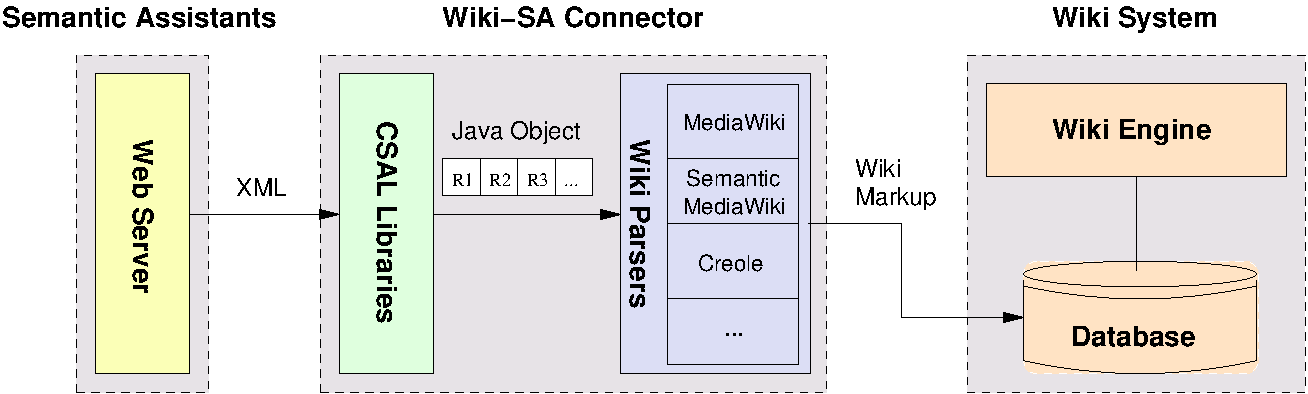
\includegraphics[width=0.7\columnwidth]{pictures/result_transform.pdf}
\caption{Transforming NLP service results to wiki markup}
\label{fig:result_transform}
\end{figure}

Following a successful NLP service execution, results are passed from the \sa server to the wiki component in form of an XML message (see Figure~\ref{list:response1} for an example). The wiki component then interprets the server's XML response and parses the message into an array of Java objects. The service result objects are eventually transformed to wiki markup by the wiki helper classes in the wiki component and prepared for the \emph{templating mechanism}. 

The templating mechanism is the process of embedding service results into wiki templates for presentation. This mechanism separates the data model from its presentation and provides the opportunity to create multiple views for a single model for different purposes. Templating is a collaborative task performed by the wiki component and the wiki plug-in. The wiki component prepares the markup by placing the results within their corresponding templates and storing them in the wiki's database. Once the wiki page is viewed by the user, the templates installed on the wiki by the \sa extension will render the template markup to generate appropriate HTML representations for NLP results, such as tables or lists. Figure~\ref{fig:result_transform} shows the workflow of the transformation of server XML response messages to MediaWiki markup.

\subsection{Wiki Component Structure}
The Wiki-SA Connector component, shown in Figure~\ref{fig:wikinlp_arch}, is technically an HTTP proxy sever written using the Java Servlet\footnote{Java Servlet API, \url{http://download.oracle.com/docs/cd/E17802_01/products/ products/servlet/2.5/docs/servlet-2_5-mr2/}} technology. As mentioned earlier, it acts as an intermediator between the \sa server, the wiki system and the user's browser by intercepting their communication. For each of these three endpoints, there exists a module in the servlet, specifically concerned with the endpoint's business logic. This way, having separate modules allows the sub-components to evolve and extend independently.

\blankline
\noindent
\textbf{Service Broker Module. }{The service broker module is the connecting point of the integration to the \sa server. Every service execution request that is received by the integration component is translated into a Java method call in this module, which in turn triggers the execution of one or multiple NLP services in the \sa server.}

\blankline
\noindent
\textbf{User Interface Module. }{This module is responsible for generating the integration user interface within a wiki environment. Since wikis are accessible through Web browsers, this module is designed to generate an HTML representation of the \sa user interface and inject it to the the user's browser using JavaScript. Injecting the user interface into the browser gives user the impression that they are still using the wiki's native interface, hence, providing a seamless experience. Through this user interface, users can find the \emph{Available Assistants} and invoke arbitrary NLP services by dynamically querying the \sa repository of service descriptions. This way, any language service that is offered by a \sa server is presented in the user interface to the user. Moreover, the generated user interface allows users to combine multiple pages of the wiki in a \emph{collection}, i.e., a list of user-selected page URLs, and invoke the NLP service on them at once.}

\blankline
\noindent
\textbf{Wiki Helper Module. }{The wiki helper module encompasses the classes required for communicating with the wiki engine. The classes in this module are responsible for providing the NLP pipelines with input data, by reading wiki pages from the database and eventually transforming the results to their corresponding template markup and storing them in the wiki repository.}

\blankline
Earlier we stated that the wiki component is responsible for maintaining and reasoning on the available wiki ontologies. This process is achieved by special ontology keeper classes that, upon each servlet bootstrapping, run over the wiki repository OWL files and create an in-memory model of the wikis, by parsing them using Prot\'{e}g\'{e}'s OWL libraries. This module also provide reasoning capabilities on wiki ontologies using the SPARQL\footnote{SPARQL Query Language for RDF, \url{http://www.w3.org/TR/rdf-sparql-query/}} language.

\subsection{Extending the Wiki Component}
One main requirement in the design of Wiki-NLP is wiki independence. With this requirement in mind, we have realized an extensible architecture where wikis can be added to the integration with little effort. The directory structure of the server-side wiki component found in \path{Clients/Wiki/src/info/semanticsoftware/semassist/client/wiki} is as follows:

\begin{description}
\item[broker] This folder contains the classes that handle the NLP service execution in the \sa server, as well as partial refinement of the results.
\item[command] This folder contains classes pertaining to the Factory Design Pattern that generate various commands that the servlet can handle. The commands themselves are implemented using the Command Design Pattern. 
\item[html] This folder contains classes that generate an HTML representation of the Wiki-NLP user interface.
\item[servlets] This folder contains the front controller classes in our proxy design.
\item[utils] This folder contains utility classes related to the wiki component, such as logging and abstract parser classes.
\item[wikihelper] This folder contains the classes pertaining to the Factory Design Pattern that generate various wiki engine instances and their corresponding parsers on the fly. Essentially, the Wiki-NLP integration provides three abstract classes, namely, \texttt{WikiHelper.java}, \texttt{WikiParser.java}, \texttt{WikiOntolgyKeeper.java}, that provide abstract methods to communicate with the wiki engine, transform the results to wiki markup and query the wiki ontology files, respectively. 
\end{description}

As the directory structure suggests, in order to introduce a new wiki engine to the integration architecture, the three mentioned classes in the \texttt{wikihelper} package needs to be extended. The current \texttt{wikihelper} package contains example classes for the MediaWiki engine. Similarly, if your wiki engine is called FooWiki, you need to create \texttt{FooWikiHelper.java}, \texttt{FooWikiParser.java} and \texttt{FooWikiOntologyKeeper.java} classes that extend the corresponding abstract classes. Once these three classes are implemented, simply extend the factory pattern in the \texttt{WikiFactory.java} by adding the name of your wiki engine to the switch statement, as shown in Figure~\ref{list:wiki_factory_extend}:

\begin{figure}[h!]
\centering
\begin{lstlisting}[language=Java,numbers=left,xleftmargin=4mm,columns=flexible]
  /** Enumeration class for wiki engines. */
  enum Wikis {mediawiki, foowiki};

  public static WikiEngine getWiki(final String engine){
    switch(Wikis.valueOf(engine.toLowerCase())){
		case mediawiki:
			return new MediaWiki();
		case foowiki:
			return new FooWiki();
		default:
			return null;
		}
  }
\end{lstlisting}
\caption{Extending the wiki factory class}
\label{list:wiki_factory_extend}
\end{figure}

Next, create a class called \texttt{FooWiki.java} and reference a singleton access to your wiki helper, parser and ontology keeper classes, just like the code in \texttt{MediaWiki.java}. Finally, place your wiki ontology \texttt{.owl} file in the \path{Clients/Wiki/WebContent/ontology-repository} folder and your wiki will show up in the list of supported engines once the servlet is restarted.
